\section{Electrons}
\label{sec:ch6_electrons}

\subsection{Reconstruction}

An electron is reconstructed from an ID track matched to an electromagnetic shower in the calorimeter.
Bremsstrahlung photons emitted in the upstream material can spread the shower energy over several clusters and alter the curvature of the electron track.
Both effects are treated in the reconstruction~\cite{ATLAS2019ElectronPerformance}:
\begin{enumerate}
    \item \textbf{Calorimeter clustering.} Neighbouring cells are grouped into topological clusters according to their signal significance above the expected noise. Clusters with a substantial electromagnetic energy fraction are used as electron seeds.
    \item \textbf{Track refitting and matching.} Electron-track candidates are refitted with a Gaussian-sum filter, in which a mixture of Gaussian components is used to describe radiative energy losses. The refitted tracks are extrapolated to the calorimeter and matched to the clusters.
    \item \textbf{Supercluster formation.} Nearby clusters are added to the seed to recover energy from bremsstrahlung. Additional clusters sharing the matched electron track can be collected over a wider region in $\phi$. The resulting variable-size supercluster is matched to the electron track to form the candidate.
\end{enumerate}
The cluster association is illustrated in Figure~\ref{fig:ch6_electron_supercluster}.
The wider collection in $\phi$ helps recover energy separated from the electron by its bending in the magnetic field.

\begin{figure}[htbp]
    \centering
    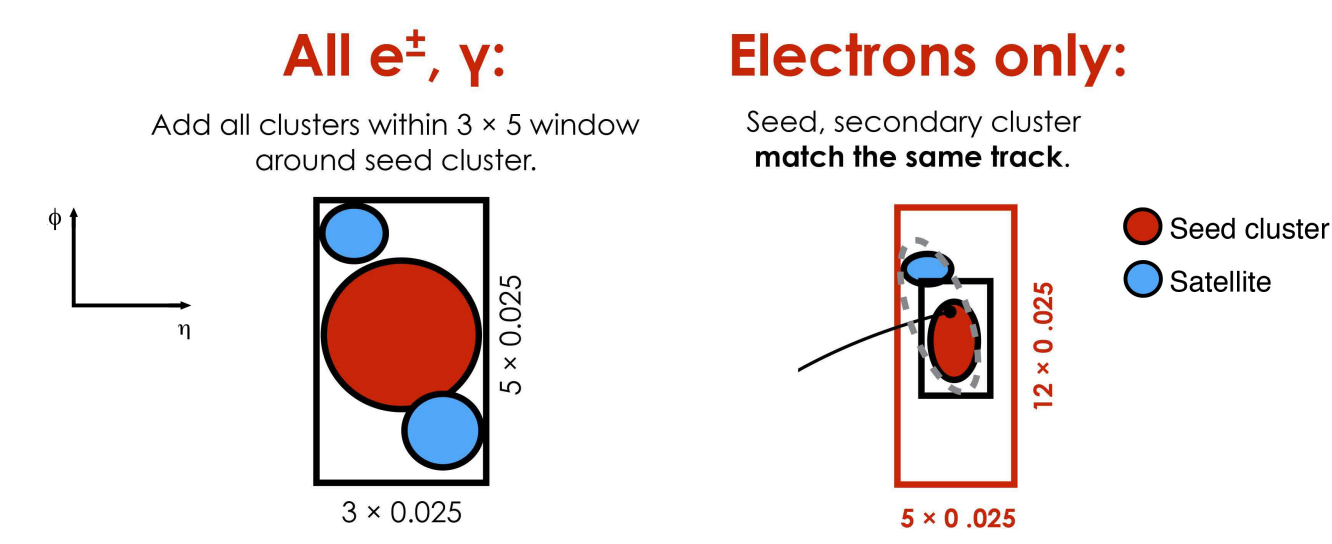
\includegraphics[width=0.75\textwidth]{output/ch6/figures/electron_superclusters.png}
    \caption{Cluster association for electron superclusters. Seed and additional clusters are shown in red and blue, respectively. Geometrically nearby clusters are collected, and a wider association is allowed for clusters sharing the electron track. The electron-relevant part of the supercluster diagram is reproduced from Ref.~\cite{ATLAS2019ElectronPerformance}.}
    \label{fig:ch6_electron_supercluster}
\end{figure}

\subsection{Identification}

Electron candidates are distinguished from hadronic showers and converted photons using a likelihood discriminant~\cite{ATLAS2019ElectronReco}.
Its inputs describe the shower shapes and hadronic leakage, the track hit content, and the agreement between the track and calorimeter measurements.
The \texttt{Loose}, \texttt{Medium} and \texttt{Tight} working points provide increasing background rejection at the cost of electron efficiency.

Baseline electrons are the initial candidates used for object counting and overlap removal.
The following requirements are imposed:
\begin{itemize}
    \item $\pT>10~\GeV$ and $|\eta|<2.47$, excluding $1.37<|\eta|<1.52$.
    \item \texttt{TightLH} identification and a calorimeter cluster passing the object-quality requirements.
    \item $|d_0|/\sigma(d_0)<5$ and $|\Delta z_0\sin\theta|<0.5~\mm$.
\end{itemize}
The impact-parameter requirements suppress electrons from displaced decays and tracks incompatible with the primary vertex.
Clusters in regions with known calorimeter defects are rejected, including the affected end-cap high-voltage regions in the 2016 data.

\subsection{Isolation}

Prompt electrons are separated from electrons inside hadronic jets by requiring little additional activity around the candidate.
Two isolation quantities are used~\cite{ATLAS2019ElectronPerformance}:
\begin{itemize}
    \item \textbf{Track isolation}: the scalar sum of the transverse momenta of nearby tracks associated with the primary vertex, excluding the electron track. The cone radius is reduced at high electron $\pT$ to limit contamination from nearby activity.
    \item \textbf{Calorimeter isolation}: the transverse energy around the electron after subtracting its own shower contribution and correcting for pile-up and shower leakage.
\end{itemize}
Baseline electrons are required to pass \texttt{Loose\_VarRad} isolation.
Signal electrons used in the analysis regions additionally pass \texttt{HighPtCaloOnly} isolation to suppress high-$\pT$ backgrounds.
Their momentum thresholds are specified with the region definitions in Chapter~\ref{chapter:event_selection}.

\subsection{Calibration}

The electron energy is calibrated for losses in upstream material, energy outside the cluster and variations in detector response~\cite{ATLAS2019ElectronPerformance}.
The residual energy scale is constrained using the reconstructed mass in $\zee$ events, and the simulated resolution is adjusted to describe the data.
Reconstruction, identification and isolation efficiencies are measured with the tag-and-probe method: one well-identified electron selects a resonance decay, and the second electron is used to test the requirement under study after background subtraction.
For a selection efficiency $\epsilon$, the scale factor is defined as
\begin{align}
    \mathrm{SF}=\frac{\epsilon_{\mathrm{data}}}{\epsilon_{\mathrm{MC}}}.
    \label{eq:ch6_efficiency_sf}
\end{align}
The appropriate scale factors are applied to simulated event weights for the electron working points used in the analysis.
